\chapter{Trade-off P/R, Curva ROC e Class. Multiclasse}
\begin{flushright}\small\textit{Lezione 6 -- 23/03/2026 -- G\'eron, Cap.\ 3 (cont.)}\end{flushright}

\section{Ricapitolo: il compromesso Precisione -- Recall}

Nella lezione precedente abbiamo visto che:
\[
P = \frac{TP}{TP + FP} \qquad R = \frac{TP}{TP + FN} \qquad F_1 = 2 \cdot \frac{P \cdot R}{P + R}
\]

Esiste un \textbf{trade-off} fondamentale: aumentare la precisione abbassa il recall e viceversa. La ragione è la \textbf{soglia di decisione} $\tau$: i classificatori come \texttt{SGDClassifier} producono un \textbf{decision score} per ogni istanza, e la soglia decide la classe predetta.

\[
\hat{y} =
\begin{cases}
+1 & \text{se } \text{score}(x) \geq \tau \\
-1 & \text{se } \text{score}(x) < \tau
\end{cases}
\]

\begin{itemize}
    \item \textbf{Alzare $\tau$} (più esigenti nel dichiarare positivo): la precisione aumenta, il recall diminuisce -- meno istanze dichiarate positive, ma quelle dichiarate sono più affidabili.
    \item \textbf{Abbassare $\tau$} (più permissivi): il recall aumenta, la precisione diminuisce -- il modello cattura più veri positivi ma anche più falsi allarmi.
\end{itemize}

\begin{exbox}[Caso A -- Video per bambini: alta precisione]
Il modello deve bloccare contenuti violenti. Non vogliamo nessun FP (un video violento classificato come sicuro). Per garantirlo, il modello diventa iperprotettivo e scarta anche cartoni innocui -- generando molti FN.

\textbf{Risultato}: Alta Precisione, Basso Recall.
\end{exbox}

\begin{exbox}[Caso B -- Telecamere anti-taccheggio: alto recall]
Nessun ladro deve sfuggire: nessun FN ammesso. La telecamera suonerà anche quando un cliente innocente mette le mani in tasca per prendere il telefono -- generando molti FP.

\textbf{Risultato}: Alto Recall, Bassa Precisione.
\end{exbox}

\section{La curva Precisione-Recall e come trovare la soglia ottimale}

Per visualizzare il trade-off su \emph{tutte} le soglie possibili, si usa la \textbf{curva Precisione-Recall (PR curve)}, ottenuta con \texttt{precision\_recall\_curve()} in Scikit-learn.

\begin{center}
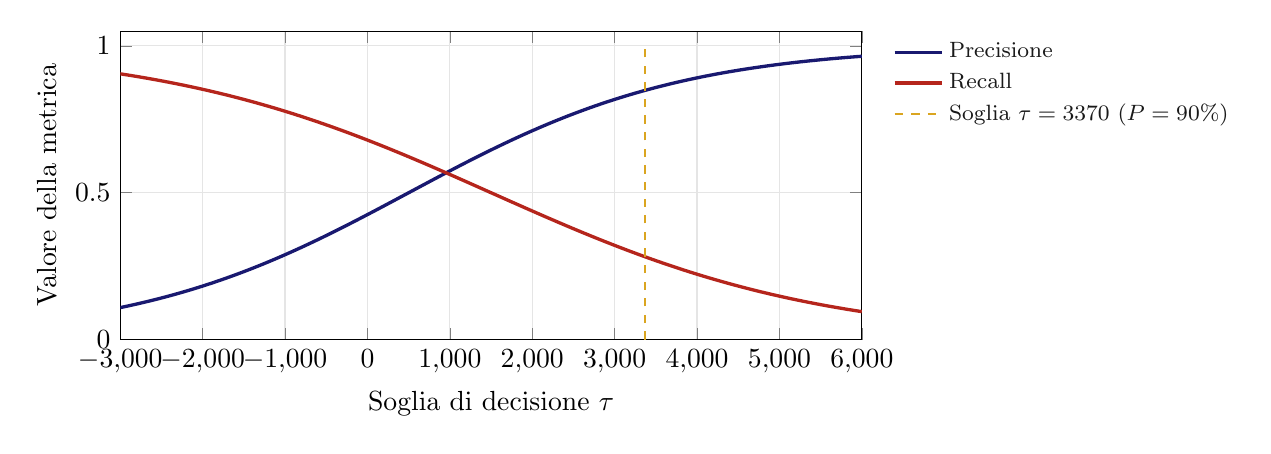
\begin{tikzpicture}
\begin{axis}[
    width=11cm, height=5.5cm,
    xlabel={Soglia di decisione $\tau$},
    ylabel={Valore della metrica},
    xmin=-3000, xmax=6000, ymin=0, ymax=1.05,
    grid=major, grid style={gray!20},
    legend pos=outer north east,
    legend style={font=\footnotesize, cells={anchor=west},
                  legend columns=1, draw=none, fill=white, fill opacity=0.9},
    legend cell align={left}
]
\addplot[very thick, MidnightBlue, domain=-3000:6000, samples=200]
    {1/(1+exp(-0.0006*(x-500)))};
\addlegendentry{Precisione}
\addplot[very thick, BrickRed, domain=-3000:6000, samples=200]
    {1 - 1/(1+exp(-0.0005*(x-1500)))};
\addlegendentry{Recall}
\addplot[thick, Goldenrod, dashed] coordinates {(3370,0)(3370,1.0)};
\addlegendentry{Soglia $\tau = 3370$ ($P = 90\%$)}
\end{axis}
\end{tikzpicture}
\end{center}

Le due curve non sono in concordanza: se una sale, l'altra scende.

\begin{notebox}[La curva P vs.\ R]
Un modo alternativo di visualizzare il trade-off è tracciare la \textbf{Precisione direttamente contro il Recall} (invece che entrambe contro la soglia). La curva ideale è vicina all'angolo in alto a destra. La precisione tende a calare bruscamente quando il recall supera circa l'80\% -- lì conviene scegliere il punto operativo.
\end{notebox}

\section{La curva ROC e l'AUC}

La curva \textbf{ROC} (\emph{Receiver Operating Characteristic}) è un altro strumento per valutare i classificatori binari. Traccia il \textbf{True Positive Rate} (recall) contro il \textbf{False Positive Rate}:

\[
TPR = \frac{TP}{TP + FN} \qquad FPR = \frac{FP}{FP + TN} = 1 - \text{Specificità}
\]

Il FPR è la percentuale di \emph{veri negativi} classificati erroneamente come positivi -- i falsi allarmi sui negativi.

\begin{center}
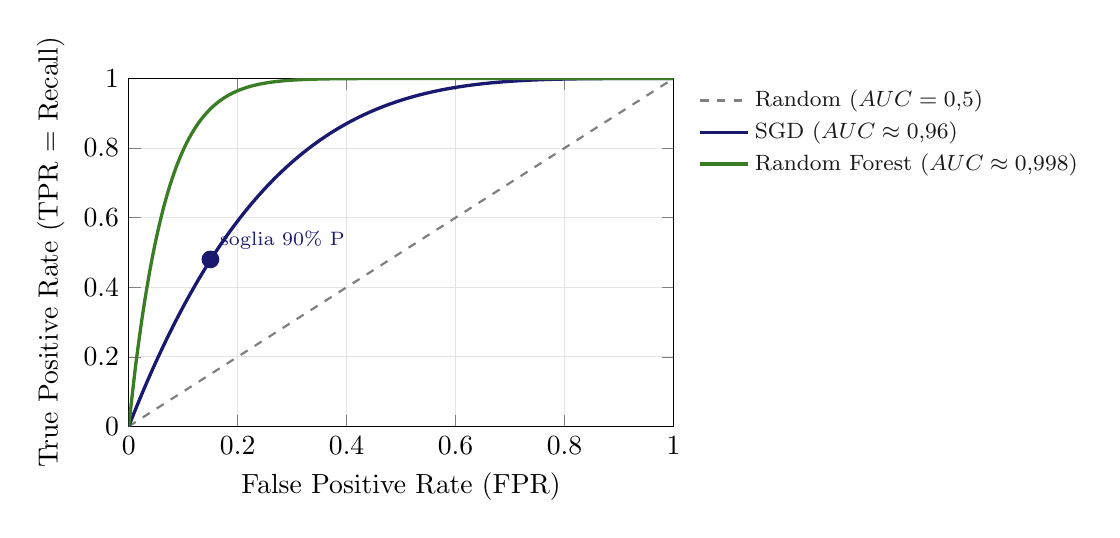
\begin{tikzpicture}
\begin{axis}[
    width=8.5cm, height=6cm,
    xlabel={False Positive Rate (FPR)},
    ylabel={True Positive Rate (TPR = Recall)},
    xmin=0, xmax=1, ymin=0, ymax=1,
    grid=major, grid style={gray!20},
    legend pos=outer north east,
    legend style={font=\footnotesize, cells={anchor=west}, 
                  legend columns=1, draw=none, fill=white, fill opacity=0.9},
    legend cell align={left}
]
\addplot[thick, gray, dashed] coordinates {(0,0)(1,1)};
\addlegendentry{Random ($AUC = 0{,}5$)}
\addplot[very thick, MidnightBlue, smooth, samples=80, domain=0:1]
    {1-(1-x)^4};
\addlegendentry{SGD ($AUC \approx 0{,}96$)}
\addplot[very thick, OliveGreen, smooth, samples=80, domain=0:1]
    {1-(1-x)^15};
\addlegendentry{Random Forest ($AUC \approx 0{,}998$)}
\addplot[mark=*, mark size=3pt, MidnightBlue] coordinates {(0.15, 0.48)};
\node[font=\scriptsize, MidnightBlue, anchor=south west] at (axis cs:0.15,0.48)
    {soglia 90\% P};
\end{axis}
\end{tikzpicture}
\end{center}

\begin{defbox}[AUC -- Area Under the Curve]
L'\textbf{AUC} sintetizza l'intera curva ROC in un numero:
\begin{itemize}
    \item $AUC = 1{,}0$ $\to$ classificatore perfetto (angolo in alto a sinistra).
    \item $AUC = 0{,}5$ $\to$ classificatore casuale (diagonale).
    \item $AUC$ = probabilità che, dato un positivo e un negativo casuali, il modello assegni allo score del positivo un valore più alto. \emph{Indipendente dalla soglia}.
\end{itemize}
\end{defbox}

\begin{exbox}[SGD vs.\ Random Forest sul 5-detector]
\begin{itemize}
    \item \textbf{SGDClassifier}: $F_1 \approx 0{,}733$, $ROC\text{-}AUC \approx 0{,}960$.
    \item \textbf{RandomForestClassifier}: $F_1 \approx 0{,}924$, $ROC\text{-}AUC \approx 0{,}998$.
\end{itemize}
Il Random Forest usa \texttt{predict\_proba()} (probabilità stimate) invece di \texttt{decision\_function()} perché non ha funzione lineare di decisione. La sua curva PR è molto più vicina all'angolo in alto a destra, confermando la superiorità.
\end{exbox}



\begin{center}
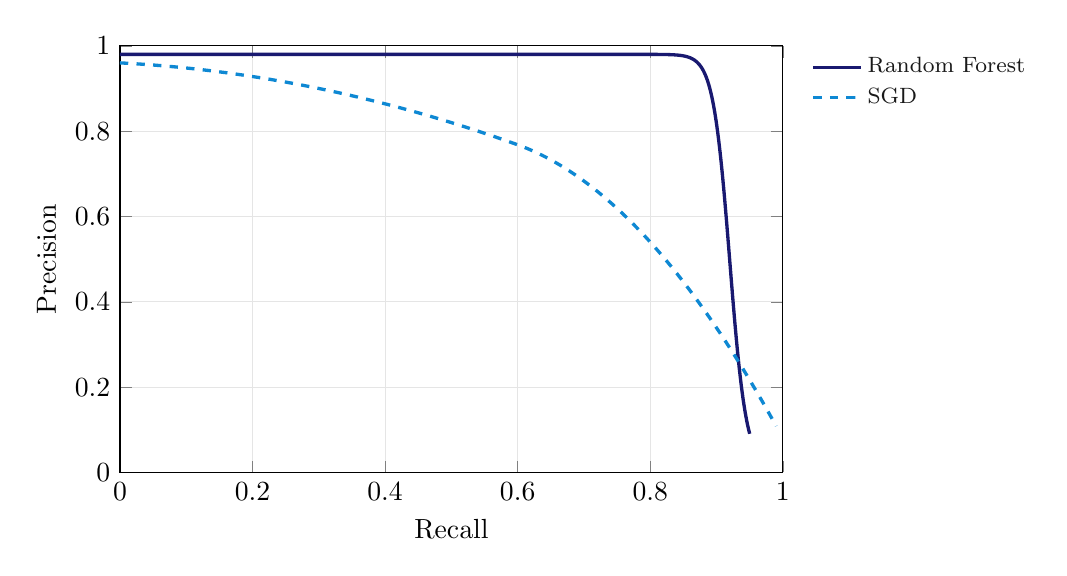
\begin{tikzpicture}
\begin{axis}[
    width=10cm, height=7cm,
    xlabel={Recall},
    ylabel={Precision},
    xmin=0, xmax=1, ymin=0, ymax=1,
    grid=major, grid style={gray!20},
    legend pos=outer north east,
    legend style={font=\footnotesize, cells={anchor=west},
                  legend columns=1, draw=none, fill=white, fill opacity=0.9},
    legend cell align={left},
    ytick={0,0.2,0.4,0.6,0.8,1.0},
    xtick={0,0.2,0.4,0.6,0.8,1.0},
    clip=false
]

\addplot[very thick, MidnightBlue, smooth, samples=300, domain=0:0.95]
    {0.97 * (1 - 1/(1 + exp(-80*(x - 0.92)))) + 0.01};
\addlegendentry{Random Forest}

\addplot[very thick, cyan!70!blue, dashed, smooth, samples=200, domain=0:0.99]
    {min(0.97, max(0.05, 0.96 - 0.08*x - 0.4*x^2 - 2.5*(max(0,x-0.6))^2))};
\addlegendentry{SGD}

\end{axis}
\end{tikzpicture}
\end{center}

\subsection{Quando usare PR curve e quando ROC}

\begin{notebox}[PR vs.\ ROC: regola pratica]
Se la classe positiva è \textbf{rara} (dataset sbilanciato) o i falsi positivi sono particolarmente costosi, preferire la \textbf{curva PR}: la ROC può sembrare ottima anche con bassa precisione, perché la massa di TN gonfia il TNR. Nel 5-detector (solo 10\% di positivi), la curva PR rivela molto più margine di miglioramento rispetto alla ROC.
\end{notebox}

\begin{center}
\renewcommand{\arraystretch}{1.3}
\begin{tabular}{@{} l p{6cm} p{6cm} @{}}
\toprule
\textbf{Metrica} & \textbf{Quando usarla} & \textbf{Quando NON usarla} \\
\midrule
Accuracy & Classi bilanciate & Classi molto sbilanciate \\
Precision & FP costoso & Quando mancare positivi è grave \\
Recall & FN costoso & Quando i FP sono costosi \\
F1 & Compromesso $P$--$R$ & Quando $P$ e $R$ hanno pesi diversi \\
ROC-AUC & Soglia ignota, classi bilanciate & Dati molto sbilanciati \\
PR-AUC & Dataset sbilanciati, FP costosi & Quando i negativi sono rilevanti \\
\bottomrule
\end{tabular}
\end{center}

\section{Classificazione Multiclasse}

Finora abbiamo lavorato in modalità binaria (``è un 5 / non è un 5''). Cosa succede se vogliamo classificare \emph{tutte e 10} le cifre?

Alcuni algoritmi sono \textbf{nativamente multiclasse}: Random Forest, Naive Bayes, KNN, MLP, Regressione Logistica. Altri sono \textbf{intrinsecamente binari}: SVM, SGD. Per usarli su più classi esistono due strategie.

\subsection{One-vs-Rest (OvR)}

Si addestrano $N$ classificatori binari, uno per classe: ``zero vs.\ tutti'', ``uno vs.\ tutti'', \ldots, ``nove vs.\ tutti''. Per classificare una nuova istanza, si eseguono tutti gli $N$ classificatori e si sceglie la classe il cui classificatore produce il \textbf{punteggio più alto}.

\begin{itemize}
    \item Costo: $O(N)$ classificatori, ognuno addestrato sull'intero training set.
    \item Default di Scikit-learn per la maggior parte degli algoritmi binari (es.\ SGD).
\end{itemize}

\subsection{One-vs-One (OvO)}

Si addestra un classificatore per \textbf{ogni coppia} di classi: ``0 vs.\ 1'', ``0 vs.\ 2'', \ldots, ``8 vs.\ 9''. Il numero totale di classificatori è:
\[
\binom{N}{2} = \frac{N(N-1)}{2}
\]
Per MNIST con 10 classi: $\frac{10 \times 9}{2} = 45$ classificatori. Per classificare, si eseguono tutti i 45 e si conta chi vince più ``duelli'' (\emph{majority vote}).

\begin{itemize}
    \item Vantaggio: ogni classificatore si allena solo su 2 classi $\to$ dataset molto più piccoli, adatto ad algoritmi che scalano male (come SVM).
    \item Svantaggio: costo quadratico $O(N^2)$ nel numero di classificatori.
    \item Default di Scikit-learn per SVM.
\end{itemize}


\section{Analisi degli errori}
Una volta selezionato un modello promettente, l'\textbf{analisi degli errori} è il passo successivo per capire come migliorarlo.

\subsection{Matrice di confusione multiclasse, normalizzata}

Con 10 classi la matrice diventa $10 \times 10$. Normalizzarla \textbf{per riga} (dividendo per il numero di istanze di ogni classe reale) permette di vedere le \textbf{percentuali} invece dei valori assoluti -- più utile quando le classi hanno numerosità diverse.

\begin{exbox}[MNIST: cosa sbaglia l'SGD?]
Dalla matrice normalizzata emerge che:
\begin{itemize}
    \item Solo l'\textbf{82\%} delle immagini di ``5'' viene classificato correttamente.
    \item Il \textbf{10\%} dei ``5'' viene scambiato per ``8''.
    \item Il \textbf{36\%} degli errori su ``7'' sono classificazioni come ``9''.
\end{itemize}
\end{exbox}

\subsection{Il trucco della diagonale}

Per far risaltare solo gli errori, si \textbf{azzera la diagonale principale} (che contiene i successi) e si visualizza la matrice come \emph{heatmap}. Le celle più luminose corrispondono agli errori più frequenti -- così si capisce subito se il modello confonde spesso, ad esempio, il ``3'' con il ``5'' o il ``4'' con il ``9''.

\begin{center}
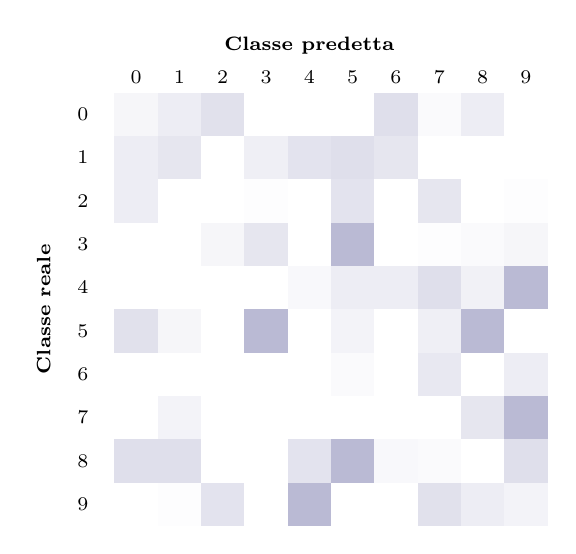
\begin{tikzpicture}[font=\scriptsize]
    \foreach \i in {0,...,9} {
        \foreach \j in {0,...,9} {
            \pgfmathsetmacro{\val}{
                (\i==\j) ? 0 :
                (\i==5 && \j==8) ? 80 :
                (\i==8 && \j==5) ? 20 :
                (\i==3 && \j==5) ? 60 :
                (\i==5 && \j==3) ? 40 :
                (\i==4 && \j==9) ? 50 :
                (\i==7 && \j==9) ? 45 :
                (\i==9 && \j==4) ? 30 :
                int(rand*15)
            }
            \pgfmathsetmacro{\col}{100-\val}
            \fill[fill=MidnightBlue!\val!white]
                (\j*0.55, -\i*0.55) rectangle (\j*0.55+0.55, -\i*0.55+0.55);
        }
    }
    \foreach \k in {0,...,9} {
        \node at (\k*0.55+0.275, 0.75) {\k};
        \node at (-0.4, -\k*0.55+0.275) {\k};
    }
    \node[font=\bfseries\scriptsize] at (2.475, 1.15) {Classe predetta};
    \node[rotate=90, font=\bfseries\scriptsize] at (-0.9, -2.2) {Classe reale};
\end{tikzpicture}
\end{center}

\subsection{Feature Engineering mirata}

Dall'analisi emergono strategie concrete:
\begin{itemize}
    \item \textbf{Raccogliere più dati} per le coppie confuse (es.\ più immagini di cifre simili all'8 che non sono 8).
    \item \textbf{Creare feature discriminative}: aggiungere il conteggio dei cerchi chiusi (8 ne ha 2, 6 ne ha 1, 5 ne ha 0) -- questo aiuta a distinguere ``5'' da ``8''.
    \item \textbf{Pre-processing}: centrare le immagini, ridurre la rotazione.
    \item \textbf{Data augmentation}: aggiungere varianti leggermente shiftate/ruotate delle immagini di training per rendere il modello più robusto alla posizione.
\end{itemize}


\section{Classificazione Multilabel}
In alcuni problemi ogni istanza può avere \textbf{più etichette contemporaneamente} -- non è una scelta mutualmente esclusiva.

\begin{exbox}[MNIST multilabel]
Per ogni cifra definiamo due label:
\begin{itemize}
    \item \textbf{``Grande''}: la cifra è $\geq 7$ (True/False).
    \item \textbf{``Dispari''}: la cifra è dispari (True/False).
\end{itemize}
Per il ``5'': output $= [False, True]$ -- non è grande, ma è dispari.\\
Per il ``7'': output $= [True, True]$ -- è grande e dispari.
\end{exbox}

Per valutare un classificatore multilabel si calcola l'\textbf{F1 per ogni label} e poi si fa la media:
\begin{itemize}
    \item \texttt{average="macro"}: media non ponderata -- tutte le label contano uguale.
    \item \texttt{average="weighted"}: media ponderata per il numero di istanze di ogni label -- enfatizza le label più frequenti.
\end{itemize}

\subsection{ClassifierChain: modellare le dipendenze tra label}

I classificatori indipendenti per ogni label ignorano le \textbf{correlazioni} tra etichette. Ad esempio, se una cifra è ``grande'' ($\geq 7$) ha il doppio delle probabilità di essere dispari. \texttt{ClassifierChain} risolve questo passando le previsioni delle label precedenti come feature aggiuntive ai modelli successivi nella catena.

\section{Classificazione Multioutput}

La \textbf{classificazione multioutput} è una generalizzazione del multilabel in cui ogni etichetta può avere \textbf{più di due valori possibili} (multiclasse per ogni output).

\begin{exbox}[Denoising di immagini MNIST]
\textbf{Input}: immagine $28 \times 28$ con rumore casuale aggiunto ai pixel.\\
\textbf{Output}: l'immagine originale pulita -- cioè 784 valori interi da 0 a 255, uno per pixel.

Questo è un task multioutput: 784 label, ciascuna con 256 valori possibili. Un \texttt{KNeighborsClassifier} addestrato su immagini rumorose (input) con le originali come target impara a ``ripulire'' nuove immagini rumorose restituendo i valori di pixel più probabili.
\end{exbox}

\begin{notebox}[Il confine tra classificazione e regressione]
Nel denoising, predire l'intensità di un pixel (da 0 a 255) potrebbe essere visto come regressione. La distinzione tra classificazione e regressione non è sempre netta: i sistemi multioutput non sono limitati alla classificazione e possono combinare label di classe e valori continui.
\end{notebox}